\documentclass[a4paper,10pt]{article}
\usepackage{amsmath}
\usepackage{enumitem}
\usepackage{booktabs}

\usepackage{tikz}
\usetikzlibrary{arrows}

\usepackage{pgfgantt}
\definecolor{blue}{HTML}{74BBC9}
\definecolor{green}{HTML}{A9D454}
\definecolor{yellow}{HTML}{F7E967}
\definecolor{red}{HTML}{F24440}
\definecolor{darkblue}{HTML}{425D69}
\definecolor{orange}{HTML}{FF9036}
\definecolor{violet}{RGB}{216,3,240}

\usepackage[backend=biber, style=numeric, sorting=none]{biblatex}
\addbibresource{paper.bib}

\title{Examining the critical path neighborhood for flexible job shop problems}
\author{Alex van Poppelen\smallskip\\
\emph{Supervisor:} Dr. J.A. Hoogeveen}

\begin{document}

\maketitle

\begin{abstract}

This is my abstract.

\end{abstract}

\tableofcontents

\section{Introduction}

\subsection{General introduction}

The Job Shop problem looks at the problem of scheduling multi operation jobs on a set of machines, where each operation in a job needs to be processed on a certain machine. The Job Shop problem is well known to be NP-hard in the strong sense, and notoriously difficult to solve even compred to other NP-hard problems.

In this paper, the Flexible Job Shop (FJS) and the Flexible Blocking Job Shop (FBJS) problems are considered. These two problems are an extension of the Job Shop and Blocking Job Shop problems where individual machines required by each operation are replaced by a number of identical machines running in parallel. Because of the need to assign operations to machines, the FJS is more complex than the classical Job Shop problem. It is therefore also known to be strongly NP-hard \cite{approxfjsp}.

In the remainder of the first section, the FJS is formally defined. The blocking constraint is also defined. In the second section, a local search approach to solve the FJS is explored. Finally, the local search approach is modified to accomodate the blocking constraints in the third section.

\subsection{Formal definition}

The Flexible Job Shop problem is defined as follows. We are given a set of $n$ jobs.

\[ \mathcal{J} = \{J_1, \dots, J_n\} \]

Each job $J_i$ consists of a fixed sequence of operations, where $o_i$ refers to the number of operations in the job:

\[ \mathcal{O}_i = \{O_{i,1}, \dots, O_{i, o_i}\} \]

Where $\mathcal{O}$ refers to the set of all operations (in this paper, individual operations will sometimes be referred to with a single subscript; in this case it will be clear from the context whether this refers to a set of job operations or a single operation). Each operation $O_{i,j}$ must be processed on a predetermined machine type.

\[ \mathcal{T} = \{T_1, \dots, T_t\} \]

Furthermore, each operation $O_{i,j}$ has a processing time $p_{i,j} > 0$ and a delay time $w_{i,j} \geq 0$. Each machine type $T_k$ has a given number of machines, defined as $m_k$. We will use $M_{k,l}$ to refer to the $l$-th machine of type $T_k$.

Machines are assumed to be continuously available from time 0, and can complete at most one operation at a time. Preemption is not allowed; the processing time $p_{i,j}$ must be uninterrupted. The delay time $w_{i,j}$ is defined as the time that must pass after operation $O_{i,j}$ is completed, before $O_{i,j + 1}$ may begin. Note that the machine $O_{i,j}$ was being processed on is immediately available.

We are interested in the following objective function.

\[ \min \{ C_\text{max} \} \]

Where $C_\text{max}$ is defined as the maximum completion time, or the time at which the last machine finished. This will be referred to as the \emph{makespan} of a schedule for the rest of this paper.

In some other literature describing the Flexible Job Shop problem, there is no concept of a machine type. Instead, each operation is defined to be processed on some subset of the set of all machines \cite{approxfjsp, ls-fbjs}. This formulation is more general than the one used in this paper.

As a result, our definition of the FJS may exclude applications in settings that combine machines suited to highly specific tasks with more generalized machines, capable of processing a larger variety of operations.

\subsection{Blocking constraint extension}

In some situations, it may be unrealistic to model a scheduling problem as a Flexible Job Shop instance. For example, a manufacturing scenario might introduce storage space constraints. The FJS assumes that a job finished processing on one machine can be removed and placed into an intermediate buffer immediately, while waiting for the next machine to become available. This assumption may be impractical, and a factory might not have room for any intermediate buffers.

We can extend the problem definition to account for these constraints. In the Flexible Blocking Job Shop problem, a machine that is finished processing a job will be blocked until that job can be moved and processed by a successive machine. Note that this definition removes the distinction between the processing times and waiting times defined above, since the machine will be blocked for the duration of the waiting time regardless of whether subsequent machines are available or not.

This definition introduces a new questions that must be resolved. For example, what happens when machine $M_{1,1}$ is blocked, waiting for machine $M_{2,1}$ to be freed, while $M_{2,1}$ is blocked waiting for $M_{1,1}$? This depends on the problem scenario, and the mechanisms in place to transfer jobs between machines. In this paper, we will assume that these mechanisms are capable of simultaneously swapping jobs between all blocked machines. Thus, any \emph{pure blocking cycles} will not cause a deadlock in the schedule.

\section{A local search approach to the FSJ}

In solving the FSJ, we are tasked with two problems. The first is to assign operations to machines. The second is to define an order on the set of operations assigned to every machine. We can choose to tackle these problems independently, or at the same time. In the independent approach, the operations would first be assigned to machines, reducing the problem to the classical Job Shop. In this paper, we will choose to tackle the problems at the same time, using a more complex schedule serialization function.

\subsection{Representation}

The classical Job Shop problem is often modeled as a disjunctive graph (for example, see \textbf{Figure \ref{fig:disjunctivegraph}}), where the directed arcs represent the precedence constraints within a job, and the undirected edges represent operations that must be processed on the same machine. By defining a direction on the edges, and making sure that these definitions result in an acyclic graph, one obtains a valid schedule for the Job Shop instance. In this case, an undirected edge represents a non-simultaneity constraint -- the two operations may be processed in any order, but not at the same time. If we wish to use the same definition for the FSJ, we are forced to assign operations to machines before directing the edges. However, that splits the problem into two parts as mentioned above, and will increase the complexity of the neighborhood. We will take another approach.

\begin{figure}[h]
\centering
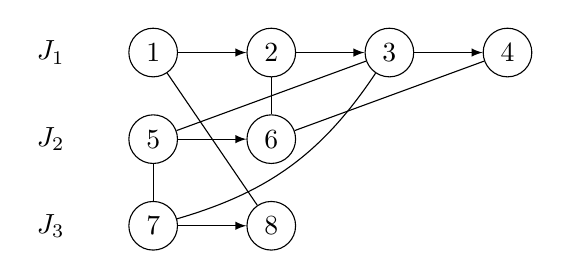
\begin{tikzpicture}

\tikzset{vertex/.style = {shape=circle,draw}}
\tikzset{arc/.style = {->,>=latex}}

% vertices
\node[vertex] (1) at  (0,0) {1};
\node[vertex] (2) at  (1.5,0) {2};
\node[vertex] (3) at  (3,0) {3};
\node[vertex] (4) at  (4.5,0) {4};
\node[vertex] (5) at  (0,-1.1) {5};
\node[vertex] (6) at  (1.5,-1.1) {6};
\node[vertex] (7) at  (0,-2.2) {7};
\node[vertex] (8) at  (1.5,-2.2) {8};

% labels
\node [left] at (-1,0) {$J_1$};
\node [left] at (-1,-1.1) {$J_2$};
\node [left] at (-1,-2.2) {$J_3$};

% arcs
\draw[arc] (1) to (2);
\draw[arc] (2) to (3);
\draw[arc] (3) to (4);
\draw[arc] (5) to (6);
\draw[arc] (7) to (8);

% edges
\draw (1) to (8);
\draw (3) to (5);
\draw [bend left=20] (3) to (7);
\draw (5) to (7);
\draw (2) to (6);
\draw (4) to (6);

\end{tikzpicture}
\caption{A disjunctive graph representing 3 jobs on 3 machines}
\label{fig:disjunctivegraph}
\end{figure}

We decide to modify the definition of an undirected edge. Instead, it will define two operations that may be processed in any order on the same machine, or independently on two different machines of the same type. Directing these edges will define the order of processing in the case the operations are on the same machine. In the case that they aren't, it only means that the start time of the second operation is equal to or greater than the start time of the first operation. This will make the serialization of a schedule more difficult, but the advantage is that generating the neighborhood will remain easy.

In our representation, we can ascertain the following information from \textbf{Figure \ref{fig:disjunctivegraph}}. There are three jobs. Operations 1 and 8 must be processed by the same machine type. Similarly, operations 2, 4, and 6 are processed on another, and 3, 5, and 7 on the last machine type.

\subsection{Serializing the schedule}

To generate a solution, all the edges in the disjunctive graph are given directions, such that the graph is acyclic. Once this has been done, it is possible to generate the corresponding schedule. The serialization function will assign operations to machines, and calculate the start time for each operation. The makespan can be determined after this process. It is important that the graph representation combined with the serialization function spans the entire set of feasible schedules. Furthermore, the serialization function should be deterministic in order to allow the local search to do its work.

To do this, we place the unscheduled operations in ordered queues for each machine type $T_k$. From these $t$ queues, we take the first operation that has no unscheduled job predecessor, and schedule it greedily into the first available machine, taking care to schedule it at the same start time or after that of the previously scheduled operation for that type. This ensures the ordering on the operations is preserved in the schedule, and conforms to the requirements that were laid out earlier in the representation section. Scheduling operations before the starting time of a previously scheduled operation on the same machine type can lead to a schedule that is actually infeasible.

If there is no operation without an unscheduled job predecessor, then there exists a cycle in the graph, and the schedule serialization fails.

We could choose to apply several tricks to generate a better schedule. Instead, we will keep the serialization as simple as possible, and allow the local search do it for us by modifying the order of the operations for each machine type.

\subsubsection{Schedule serialization example}

\begin{figure}[h]
\centering
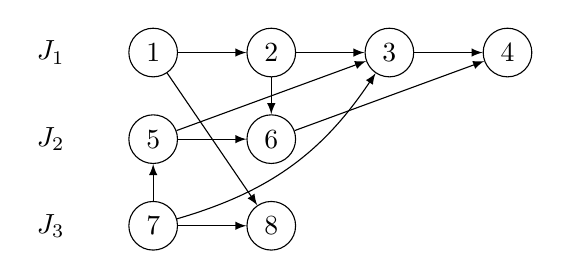
\begin{tikzpicture}

\tikzset{vertex/.style = {shape=circle,draw}}
\tikzset{arc/.style = {->,>=latex}}

% vertices
\node[vertex] (1) at  (0,0) {1};
\node[vertex] (2) at  (1.5,0) {2};
\node[vertex] (3) at  (3,0) {3};
\node[vertex] (4) at  (4.5,0) {4};
\node[vertex] (5) at  (0,-1.1) {5};
\node[vertex] (6) at  (1.5,-1.1) {6};
\node[vertex] (7) at  (0,-2.2) {7};
\node[vertex] (8) at  (1.5,-2.2) {8};

% labels
\node [left] at (-1,0) {$J_1$};
\node [left] at (-1,-1.1) {$J_2$};
\node [left] at (-1,-2.2) {$J_3$};

% arcs
\draw[arc] (1) to (2);
\draw[arc] (2) to (3);
\draw[arc] (3) to (4);
\draw[arc] (5) to (6);
\draw[arc] (7) to (8);

% edges
\draw[arc] (1) to (8);
\draw[arc] (5) to (3);
\draw[arc] [bend right=20] (7) to (3);
\draw[arc] (7) to (5);
\draw[arc] (2) to (6);
\draw[arc] (6) to (4);

\end{tikzpicture}
\caption{An acyclic directed graph representing a schedule}
\label{fig:dag}
\end{figure}

Consider the acyclic directed graph in \textbf{Figure \ref{fig:dag}}. The serialization function would set up three ordered queues:

\[ T_1\colon O_1 \rightarrow O_8 \]
\[ T_2\colon O_2 \rightarrow O_6 \rightarrow O_4 \]
\[ T_3\colon O_7 \rightarrow O_5 \rightarrow O_3 \]

Since operation $O_2$ has an unscheduled job predecessor, the algorithm would schedule $O_1$ or $O_7$ at time 0 on their respective machines first. After $O_1$ is scheduled, $O_2$ would become available to be scheduled at time $p_{1,1} + w_{1,1}$ or later. The algorithm continues until all the queues are empty or a cycle has been found. In the first case, the makespan is easily determined as the largest finish time for all the operations.

\subsubsection{Waiting cycle}

The acyclic property of the directed graph is crucial to the serialization process. It determines whether a configuration results in a feasible schedule or not. Suppose, using the above example, the arcs were modified to produce the following different queues for $T_1$ and $T_3$:

\[ T_1\colon O_8 \rightarrow O_1 \]
\[ T_3\colon O_5 \rightarrow O_3 \rightarrow O_7 \]

In this case, a cycle exists from $O_1 \rightarrow O_3 \rightarrow O_7 \rightarrow O_8$, and back to $O_1$. When the scheduler tries to serialize this configuration, it schedules $O_5$ as normal. Then it has $O_8$ to schedule on $T_1$, and $O_3$ on $T_3$. However, $O_8$ cannot be scheduled until $O_7$ is scheduled, and $O_3$ cannot be scheduled until $O_1$ (and $O_2$) is sceduled. This will be referred to as a \emph{waiting cycle}.

\subsection{Critical path neighborhood}

For the classical Job Shop problem, a commonly used neighborhood is the set of all critical block swaps. The critical block swap is a reversal of an edge on the longest path of the disjunctive graph. This neighborhood is quite small, focusing on the operations that influence the length of the makespan. More importantly, the neighborhood is guaranteed to consist only of other acyclic graphs, or feasible solutions \cite{simulatedannealingjsp}.

For the FJS, we can define the longest path in a similar manner. Whereas the longest path for the classical Job Shop problem was also chronologically sequential in terms of the generated schedule, this is no longer necessarily the case for the FJS. We must also consider operations on the same machine type, scheduled on different machines. For example, consider the operations $O_{1,1}$ and $O_{2,2}$ from different jobs that must be scheduled on machines of type $T_k$, connected by a directed edge from $O_{1,1}$ to $O_{2,2}$. Suppose $O_{1,1}$ has been scheduled at time $t_1$ on machine $M_{k,1}$ due to a precedence constraint. Further suppose that machine $M_{k,2}$ is available from some time $t_2 < t_1$. However, the serialization function is forced to schedule $O_{2,2}$ on $M_{k,2}$ at time $t_1$ anyway. In this scenario, we would like to reverse the order of the arc between $O_{1,1}$ and $O_{2,2}$, so that $O_{2,2}$ may be scheduled earlier and therefore potentially decrease the length of the longest path.

Therefore, we construct our neighborhood by considering operations $v$ and $w$ such that:

\begin{itemize}
	\item $v$ and $w$ have both been scheduled consecutively on the same machine
	\item $v$ and $w$ have been scheduled on different machines of the same type at the same time
\end{itemize}

\subsubsection{Applying the swap}

Let's consider the ordered queues containing the set of operations on a machine type, as defined by the acyclic directed graph corresponding to a feasible schedule. In the classical Job Shop case, a critical block swap identifies two consecutively scheduled nodes on a machine. These two nodes are necessarily consecutive in the queue, as well. In the FJS problem, this is no longer necessarily the case, since operations in between may have been scheduled on other machines of the same type. If one of these other operations is of the same job as either of the selected nodes, simply reversing the directed edge between the two nodes will lead to one or more cycles.

\begin{figure}[h]
\centering
\begin{ganttchart}[
		x unit=0.7cm,
		y unit chart=0.7cm,
		canvas/.style={draw=none,fill=none},
		vgrid,
		vgrid={*1{draw=black!12}},
		inline,
		group/.style={draw=none,fill=none},
		bar top shift=0.1,
		bar height=0.8,
		y unit title=0.5cm,
		title/.style={draw=none,fill=none},
		include title in canvas=false,
	]{-1}{12}

	\gantttitle{0}{2}
	\gantttitle{2}{2}
	\gantttitle{4}{2}
	\gantttitle{6}{2}
	\gantttitle{8}{2}
	\gantttitle{10}{2}
	\gantttitle{12}{2} \\

	\ganttgroup[inline=false]{$M_{1,1}$}{0}{1}
	\ganttbar[bar/.style={fill=yellow}]{2,12}{3}{4}
	\ganttbar[bar/.style={fill=blue}]{1,10}{6}{7} \\

	\ganttgroup[inline=false]{$M_{1,2}$}{0}{1}
	\ganttbar[bar/.style={fill=blue}]{1,9}{2}{5}
	\ganttbar[bar/.style={fill=yellow}]{2,13}{6}{8} \\

	\ganttgroup[inline=false]{$M_{2,1}$}{0}{1}
	\ganttbar[bar/.style={fill=blue}]{1,8}{0}{1}
	\ganttbar[bar/.style={fill=yellow}]{2,14}{9}{11} \\
	
	\ganttgroup[inline=false]{$M_{3,1}$}{0}{1}
	\ganttbar[bar/.style={fill=yellow}]{2,11}{0}{2}

\end{ganttchart}
\caption{A flexible job shop schedule}
\label{fig:sch-swap}
\end{figure}

Consider the schedule shown in \textbf{Figure \ref{fig:sch-swap}}. The ordered queue for $T_1$ that generated this schedule follows:

\[ O_{1,9} \rightarrow O_{2,12} \rightarrow O_{1,10} \rightarrow O_{2,13} \]

We wish to swap the order of operations $O_{1,9}$ and $O_{2,13}$, both on the critical path. Simply swapping their places leads to cycles, since the job operations will be out of order. We can resolve this situation by reversing a few more arcs, to achieve the following ordering.

\[ O_{2,12} \rightarrow O_{2,13} \rightarrow O_{1,9} \rightarrow O_{1,10} \]

This can be done by incrementely swapping both target operations inwards, stopping if the swap would occur with another operation of the same job, or if the two target operations have switched order. This preserves the order among all operations exluding the two targets. Although this swap is now bounded by $O(n)$ in the worst case, in practice it will be much faster, since the two operations being swapped are chronologically sequential. It can be shown that this type of swap for two operations on the longest path can always be done without creating any cycles within the machine type.

Suppose the method above was not able to swap two operations, $O_{i,a_1}$ and $O_{j,b_2}$ for $i \neq j$. Then there exist operations $O_{i,a_2}$ and $O_{j,b_1}$ with $a_1 < a_2$ and $b_1 < b_2$ such that the ordered queue is equivalent to the following:

\[ \dots \rightarrow O_{i,a_1} \rightarrow \dots \rightarrow O_{i,a_2} \rightarrow \dots O_{j,b_1}
\rightarrow \dots \rightarrow O_{j,b_2} \rightarrow \dots \]

This configation does not allow for the above swap without changing the order between the two inner operations, since it would create a cycle. However, it is easy to see that such an ordering will never create a schedule such that $O_{i,a_1}$ and $O_{j,b_2}$ are consecutive on the longest path, since operation $O_{j,b_1}$ has a non-zero processing time, and cannot be scheduled until after or equal to the finish time of $O_{i,a_1}$ due to $O_{i,a_2}$.

\subsubsection{Infeasible solutions}

The critical path neighborhood for the classical Job Shop is guaranteed to consist of only feasible schedules (acyclic graphs), a very nice result from Van Laarhoven et al \cite{simulatedannealingjsp}. Unfortunately, this is not the case for the Flexible Job Shop. We have slightly modified the swap operation to ensure no waiting cycles within a machine type are created. However, this does not guarantee no waiting cycles in the entire graph are generated. Consider the schedule shown in \textbf{Figure \ref{fig:sch-cycle}}, where colors correspond to jobs.

\begin{figure}[h]
\centering
\begin{ganttchart}[
		x unit=0.7cm,
		y unit chart=0.7cm,
		canvas/.style={draw=none, fill=none},
		vgrid,
		vgrid={*1{draw=black!12}},
		inline,
		group/.style={draw=none, fill=none},
		bar top shift=0.1,
		bar height=0.8,
		y unit title=0.5cm,
		title/.style={draw=none, fill=none},
		%title label/.style={align=left},
		include title in canvas=false,
	]{655}{669}

	\gantttitle{656}{2}
	\gantttitle{658}{2}
	\gantttitle{660}{2}
	\gantttitle{662}{2}
	\gantttitle{664}{2}
	\gantttitle{666}{2}
	\gantttitle{668}{2} \\

	\ganttgroup[inline=false]{$M_{1,1}$}{656}{657}
	\ganttbar[bar/.style={fill=blue}]{1225}{656}{664}
	\ganttbar[bar/.style={fill=green}]{1298}{665}{668} \\

	\ganttgroup[inline=false]{$M_{1,2}$}{656}{657}
	\ganttbar[bar/.style={fill=yellow}]{905}{657}{665} \\

	\ganttgroup[inline=false]{$M_{1,3}$}{656}{657}
	\ganttbar[bar/.style={fill=darkblue}]{1009}{657}{658}
	\ganttbar[bar/.style={fill=red}]{1055}{659}{661}
	\ganttbar[bar/.style={fill=orange}]{1249}{662}{668} \\

	\ganttgroup[inline=false]{$\dots$}{656}{657} \\

	\ganttgroup[inline=false]{$M_{4,1}$}{656}{657}
	\ganttbar[bar/.style={fill=darkblue}]{1010}{660}{663} \\

	\ganttgroup[inline=false]{$M_{4,4}$}{656}{657}
	\ganttbar[bar/.style={fill=green}]{1297}{660}{660}

\end{ganttchart}
\caption{A flexible job shop schedule}
\label{fig:sch-cycle}
\end{figure}

The acyclic directed graph that generated this schedule could have the following partial ordered queue for machine type $T_1$:

\[ \dots \rightarrow O_{1225} \rightarrow O_{905} \rightarrow O_{1009} \rightarrow O_{1055} \rightarrow O_{1249} \rightarrow O_{1298} \rightarrow \dots \]

The ordering on $T_4$ could have $O_{1010}$ placed before $O_{1297}$. Suppose that $O_{1225}$ and $O_{1298}$ were on the critical path, and have been selected for a swap. Applying the swap operation as described above would simply move $O_{1298}$ to the front of the chain. A cycle is created, from $O_{1010} \rightarrow O_{1297} \rightarrow O_{1298} \rightarrow O_{1009}$ and back to $O_{1010}$.

In this case, we could perform checks and swap the two operations after the offending $O_{1009}$. However, correcting for one cycle could potentially lead to another, and the operation would become very expensive. In practice, these kinds of cycles rarely occur, and it is better to simply reverse the swap and allow the heuristic to try something else.

\subsection{Computational results}

Unfortunately, given the more restrictive formulation, there are no benchmark instances or results from the literature to compare to. Classical Job Shop instances do fit in our formulation, so a few have been included just for reference. These instances, \emph{ft06}, \emph{ft10}, and \emph{ft20} were generated by Fisher and Thompson (available on the web \cite{jobshopinfo}).

The next set of instances come from a previous project on exact methods for the FJS \cite{cijvat}, therefore including the optimal values. These instances are labeled \emph{c1 -- c19}. It should be noted that in almost all of these instances, the optimal makespan is equal to the maximum job makespan. This makes it easy to prove optimality, and also much easier to find an optimum.

The rest of the instances were generated using a random instance generator built for this purpose. These are labeled \emph{v10 -- v43}. The optimal makespans for these instances is unknown. However, they do provide insight into the convergence behavior, especially when compared between instances.

The local search was implemented in C, using the GCC compiler with the -O3 flag. The times listed are for an Intel Core i3 M370 @ 2.40 Hz. These results can be examined in \textbf{Table \ref{table:fjs}}.

\begin{table}[h]
\centering
\small
\begin{tabular}{@{\bfseries}rrrrrrrrrrrr}
	\toprule
	\multicolumn{4}{c}{Instance} & \multicolumn{2}{c}{Properties} && \multicolumn{5}{c}{Results} \\
	\cmidrule(r){1-4} \cmidrule(lr){5-6} \cmidrule(lr){8-12}
	\normalfont{name} & $|\mathcal{J}|$ & $|\mathcal{T}|$ & $|\mathcal{M}|$ & $\max C_\text{job}$ &
	$C_\text{opt}$ && $\alpha$ & restarts & $\bar{C}$ & $C_\text{best}$ & $\bar{t}$ \\
	\midrule
	ft06 &  6 &  6 &  6 &   47 &   55 &&    0.9 & 1 &   55 &   55 &    0 \\
	ft10 & 10 & 10 & 10 &  655 &  930 &&    0.9 & 5 &  954 &  941 &    2 \\
	     &    &    &    &      &      &&   0.99 & 5 &  943 &  938 &   18 \\
	     &    &    &    &      &      &&  0.999 & 5 &  933 &  930 &  182 \\
	ft20 & 20 &  5 &  5 &  387 & 1165 &&    0.9 & 5 & 1215 & 1186 &    1 \\
	     &    &    &    &      &      &&   0.99 & 5 & 1182 & 1178 &   13 \\
	     &    &    &    &      &      &&  0.999 & 5 & 1170 & 1165 &  130 \\[2ex]
	c1   &  4 &  2 &  4 &   34 &   34 &&    0.9 & 1 &   34 &   34 &    0 \\
	c2   &  4 &  2 &  4 &   53 &   53 &&    0.9 & 1 &   53 &   53 &    0 \\
	c3   &  4 &  2 &  4 &  133 &  143 &&    0.9 & 1 &  143 &  143 &    0 \\
	c4   &  6 &  2 &  4 &   52 &   57 &&   0.99 & 5 &   57 &   57 &    2 \\
	c5   &  6 &  2 &  4 &  105 &  113 &&   0.99 & 5 &  113 &  113 &    2 \\
	c6   &  6 &  2 &  4 &  205 &  225 &&   0.99 & 5 &  225 &  225 &    2 \\
	c7   &  4 &  3 &  9 &   39 &   39 &&    0.9 & 1 &   39 &   39 &    0 \\
	c8   &  4 &  3 &  9 &   64 &   64 &&    0.9 & 1 &   64 &   64 &    0 \\
	c9   &  4 &  3 &  9 &  138 &  138 &&    0.9 & 1 &  138 &  138 &    0 \\
	c10  &  6 &  3 &  9 &   50 &   50 &&    0.9 & 1 &   50 &   50 &    0 \\
	c11  &  6 &  3 &  9 &  103 &  103 &&    0.9 & 1 &  103 &  103 &    0 \\
	c12  &  6 &  3 &  9 &  204 &  204 &&    0.9 & 1 &  204 &  204 &    0 \\
	c13  &  8 &  3 &  9 &  337 &  337 &&    0.9 & 5 &  337 &  337 &    0 \\
	c14  &  8 &  3 &  9 &  705 &  705 &&    0.9 & 5 &  705 &  705 &    0 \\
	c15  &  8 &  3 &  9 & 1458 & 1458 &&    0.9 & 5 & 1458 & 1458 &    0 \\
	c16  & 10 &  4 & 16 &  405 &  405 &&    0.9 & 5 &  405 &  405 &    0 \\
	c17  & 10 &  4 & 16 &  955 &  955 &&    0.9 & 5 &  955 &  955 &    0 \\
	c18  & 10 &  4 & 16 & 1621 & 1621 &&    0.9 & 5 & 1621 & 1621 &    0 \\
	c19  & 15 &  5 & 25 & 2631 & 2631 &&    0.9 & 5 & 2631 & 2631 &    0 \\[2ex]
	v20  &  8 &  2 &  4 &      &      &&    0.9 & 5 &      &      &      \\
	v30  & 16 &  2 &  4 &  666 &      &&    0.9 & 5 & 2382 & 2381 &   10 \\
	     &    &    &    &      &      &&   0.99 & 5 & 2381 & 2381 &  102 \\
	v31  & 16 &  2 &  8 &  566 &      &&    0.9 & 5 &  963 &  961 &   12 \\
	     &    &    &    &      &      &&   0.99 & 5 &  960 &  959 &  126 \\
	v32  & 16 &  4 &  8 &  655 &      &&    0.9 & 5 & 1119 & 1116 &   11 \\
	     &    &    &    &      &      &&   0.99 & 5 & 1112 & 1111 &  116 \\
	\bottomrule
\end{tabular}
\caption{Computational results for the FJS}
\label{table:fjs}
\end{table}

Most of the parameters in the table are self-explanatory. $\alpha$ is the cooling parameter. It is responsible for lowering the tempterature of the simulated annealing process. A value closer to 1 means the temperature cools slower, and thus the heuristic searches longer. The restarts column indicates how many times the temperature was reset. This entire process was repeated five times for every instance, to provide an average best solution found ($\bar{C}$) and the average running time ($\bar{t}$).

\subsection{Analysis}

For the Job Shop instances (\emph{ft06}, \emph{ft10}, and \emph{ft20}), the code as well as previous results in literature \cite{simulatedannealingjsp}. This gives us confidence that the code is robust.

The series of instances from the previous project (\emph{c1 -- c19}) are largely uninteresting, due to there being too few jobs in relation to machines. Interestingly, the few instances whose optimal makespans were larger than the lower bound given by the job makespans gave the search more trouble, despite being much smaller than some of the other instances. In several cases, the search failed to find an optimal solution despite the restarts, being very slightly off. However, this was averaged out by the other results. It should be noted that there were several instances of the algorithm becoming stuck, with the only neighborhood solution available being infeasible. This is very rare, but it highlights the importance of random restarts, when using the critical path neighborhood for the FJS.

For the other instances, we see that the algorithm converges very quickly. More searching failed to find solutions significantly below the best solutions found almost immediately. This indicates the critical path neighborhood works very well for the Flexible Job Shop problem. As the solution improves, the size of the neighborhood becomes smaller and smaller. This leads to very fast converging behavior.

It is also interesting to note that the amount of machine types and total machines have little to do with the "difficulty" of the instance. The algorithm converged equally quickly for all machine type configurations, with the amount of jobs and operations held constant.

\section{A local search approach to the FBSJ}

\subsection{Serialization}

Intuitively, we can use the exact same representation and critical path neighborhood for the FBJS problem as for the FJS. The serialization function will have to be modified slightly to account for the blocking constraints. This is relatively simple -- the greedy algorithm will simply mark a machine as blocked after scheduling an operation, and unmark it when its successor is scheduled.

As mentioned in the introduction, the blocking constraint introduces new types of cycles.

\subsubsection{Pure blocking cycle}

An example of a pure blocking cycle is one where operation $O_{j_1,a}$ has been scheduled on machine $M_{t_1,m}$ and $O_{j_2,b}$ has been scheduled on $M_{t_2,n}$. Both of these machines are now blocked. Suppose there are no other available machines for machine types $T_{t_1}$ and $T_{t_2}$, and the scheduler now encounters $O_{j_2,b+1}$ to be scheduled on type $T_{t_1}$ and $O_{j_1,a+1}$ for $T_{t_2}$. Since the only possible machines for these types are blocked, this can only be resolved if the two machines can swap jobs simultaneously, as described in the introduction. Since we allow for blocking with swaps, the scheduler must recognize this type of cycle and schedule the two (or more) operations simultaneously.

Unfortunately, this cycle does not show up in our disjunctive graph representation, so we cannot detect it using traditional graph algorithms. We can choose to extend our representation, and indeed this may be the most complete choice. However, the scheduler will encounter maximally 1 operation to be scheduled on each machine type at once. Thus these cycles are guaranteed to be small and quite simple. By running through the blocked operations in $O(n^3)$ time, the scheduler can reliably identify these cycles and resolve them.

\subsubsection{Variable cycle}

A variable cycle is a mix of waiting and blocking. For example, suppose operation $O_{j_1,a}$ has been scheduled on machine $M_{T_i, k}$, the only available machine of its type. It is now blocked, and cannot schedule the next operation, $O_{j_2,b}$. However, this means $T_j$ cannot schedule its next operation, $O_{j_2,b + 1}$. $O_{j_1,a + 1}$ is unscheduled and ordered after $O_{j_2,b + 1}$, creating a deadlock. One machine is blocked, while the other is waiting.

This is an infeasible solution and cannot be resolved without reversing some edges. In this paper, we simply reverse the operation leading to this configuration, and try something else.

\subsection{Naive shift neighborhood}

There is little literature on the FBJS, and as a result there are even few benchmark instances and results. In any case, these would not be applicable here due to the less generalized formulation we have used. To better assess the critical path neighborhood, we introduce a naive shift neigbhorhood for comparison.

In this neighborhood, we take a random operation of a random machine type, and shift it a random number of (permissible) places left or right. It may also take all of operations of the job this operation belongs to, and shift them all an individually random number of places left. The blocking constraint means that the operations belonging to a job must be executed as close together as possible. In this sense, it makes sense to move these operations as a unit, rather than individually.

While this neighborhood somewhat takes the nature of blocking and jobs into account, it doesn't use any information concerning the critical path, waiting and/or blocking times, or other useful properties. It is therefore referred to as a naive neighborhood.

\subsection{Computational results}

The same instances are used as before. A new column, containing the best non-blocking solution for the instance, is added for comparison.

\begin{table}[h]
\centering
\small
\begin{tabular}{@{\bfseries}rrrrrrrrrrrrr}
	\toprule
	& FJS & FBJS & && \multicolumn{2}{c}{Critical Path} &&
	\multicolumn{2}{c}{Naive shift} && \multicolumn{2}{c}{Both} \\
	\cmidrule(lr){2-2} \cmidrule(lr){3-3} \cmidrule(lr){6-7}
	\cmidrule(lr){9-10} \cmidrule(lr){12-13}
	\normalfont{name} & $C_\text{best}$ & $C_\text{opt}$ & $\alpha$ && $\bar{C}$ & $C_\text{best}$ &&
	$\bar{C}$ & $C_\text{best}$ && $\bar{C}$ & $C_\text{best}$ \\
	\midrule
	ft06 &   55 &   63 &  0.99 &&  102 &   95 &&   64 &   63 &&   66 &   63 \\
	ft10 &  930 & 1068 &   0.9 && 2183 & 1931 && 1507 & 1436 && 1464 & 1415 \\
	     &      &      &  0.99 && 2139 & 1931 && 1444 & 1353 && 1413 & 1349 \\
	     &      &      & 0.999 && 2366 & 2028 && 1380 & 1281 && 1371 & 1292 \\
	ft20 & 1165 &      &   0.9 && 2476 & 2406 && 1957 & 1866 && 1935 & 1869 \\
	     &      &      &  0.99 && 2454 & 2348 && 1840 & 1814 && 1860 & 1840 \\
	     &      &      & 0.999 && 5 & 1170 && 1165 &  130 &&   & \\[2ex]
	c1   &   34 &      &  0.99 &&   66 &   62 &&   37 &   37 &&   37 &   37 \\
	c2   &   53 &      &  0.99 &&   88 &   75 &&   65 &   65 &&   65 &   65 \\
	c3   &  143 &      &  0.99 &&  206 &  206 &&  180 &  180 &&  180 &  180 \\
	c4   &   57 &      &  0.99 &&  116 &  109 &&   94 &   92 &&   91 &   90 \\
	c5   &  113 &      &  0.99 &&  247 &  215 &&  180 &  170 &&  175 &  170 \\
	c6   &  225 &      &  0.99 &&  502 &  434 &&  365 &  360 &&  360 &  353 \\
	c7   &   39 &      &  0.99 &&   39 &   39 &&   39 &   39 &&   39 &   39 \\
	c8   &   64 &      &  0.99 &&   64 &   64 &&   64 &   64 &&   64 &   64 \\
	c9   &  138 &      &  0.99 &&  138 &  138 &&  138 &  138 &&  138 &  138 \\
	c10  &   50 &      &  0.99 &&   50 &   50 &&   50 &   50 &&   50 &   50 \\
	c11  &  103 &      &  0.99 &&  170 &  116 &&  106 &  106 &&  106 &  106 \\
	c12  &  204 &      &  0.99 &&  265 &  210 &&  208 &  208 &&  208 &  208 \\
	c13  &  337 &      &  0.99 &&  557 &  524 &&  467 &  458 &&  393 &  389 \\
	c14  &  705 &      &  0.99 && 1203 & 1036 &&  866 &  833 &&  797 &  788 \\
	c15  & 1458 &      &  0.99 && 2556 & 2258 && 1789 & 1666 && 1508 & 1493 \\
	c16  &  405 &      &  0.99 &&  519 &  483 &&  444 &  429 &&  405 &  405 \\
	c17  &  955 &      &  0.99 && 1257 & 1009 &&  962 &  955 &&  955 &  955 \\
	c18  & 1621 &      &  0.99 && 2314 & 2131 && 1710 & 1688 && 1621 & 1621 \\
	c19  & 2631 &      &  0.99 && 4568 & 3973 && 4365 & 4049 && 2631 & 2631 \\[2ex]
	v20  &      &      &   0.9 &&  571 &  540 &&  494 &  476 &&  438 &  423 \\
	     &      &      &  0.99 &&  527 &  517 &&  447 &  421 &&  424 &  418 \\
	v21  &      &      &   0.9 &&  331 &  293 &&  277 &  254 &&  218 &  215 \\
	     &      &      &  0.99 &&  327 &  291 &&  213 &  209 &&  198 &  194 \\
	v22  &      &      &   0.9 &&  419 &  387 &&  326 &  314 &&  294 &  284 \\
	     &      &      &  0.99 &&  393 &  369 &&  293 &  281 &&  273 &  262 \\
	v30  & 2381 &      &   0.9 && 4210 & 4068 && 5969 & 5856 && 3546 & 3438 \\
	     &      &      &  0.99 && 4200 & 4154 && 5591 & 5411 && 3287 & 3147 \\
	v31  &  959 &      &   0.9 && 1658 & 1573 && 4303 & 4133 && 1702 & 1635 \\
	     &      &      &  0.99 && 1688 & 1632 && 3772 & 3712 && 1646 & 1617 \\
	v32  & 1111 &      &   0.9 && 5 & 1119 && 1116 &   11 &&   & \\
	     &      &      &  0.99 && 2629 & 2601 && 1111 &  116 &&   & \\
	\bottomrule
\end{tabular}
\caption{Computational results for the FBJS}
\label{table:fbjs}
\end{table}

\subsection{Analysis}

It is immediately apparent that for almost all instances, the critical path neighborhood fails to search large portions of the solution space. It quickly converges to a certain makespan, and then fails to improve on it -- even if it is very far off the optimal solution. Sometimes, this makespan is even worse than one reached by the naive shift neighborhood. Neither of the neighborhoods seem to reach good solutions at all, except in the case of an excess of machines. The combination of the two neighborhoods performs better than either of the neighborhoods alone, but the solution quality and speed of convergence still leave much to be desired.

Analyzing the critical path neighborhood reveals a very high percentage of infeasible solutions in the neighborhood. The critical path neighborhood is quite small, which is a strength in the FJS case. However, this means it explores very little of the solution space, and the search quickly becomes stuck due to the large amounts of infeasible solutions. Combining the two neighborhoods improved the search somewhat. In any case, it appears as though moving individual operations on the critical path simply creates infeasible solutions in too many cases.

The blocking constraint means that good solutions will have jobs packed tightly together, in order to minimize the times that machines are blocked instead of processing. Attempting to move one operation out of a tightly packed job to a new time in the schedule will almost inevitably lead to a variable cycle, and an infeasible solution. This is most likely the cause of the failure of the critical path neighborhood when applied to the Blocking Job Shop. It is clear a different approach is needed, perhaps one that looks at entire jobs instead of individual operations.

\section{Conclusions and further research}

We have examined the critical path neighborhood in conjunction with a local search for the Flexible Job Shop and Flexible Blocking Job Shop problems.

For the Flexible Job Shop problem, the critical path neighborhood is a very effective search mechanism, performing nearly as well as it does for the classical Job Shop. It doesn't provide the same feasibility guarantees, but in practice this is hardly an issue. With a small number of random restarts, the search will almost invariably find a good solution, and converge very quickly. The strength of this neighborhood lies in its small size and the clever use of the problem characteristics.

These strengths quickly turn into weaknesses when the blocking constraint is added to the problem. The critical path neighborhood fails to effectively search the solution space, and performs more poorly than even the most primitive neighborhoods. Even when combined with a different neighborhood to help it explore different areas of the solution space, it fails to make a significant impact on the solution quality and the rate of convergence. A different approach is needed, one that takes important relationships between operations of the same job into account.

There are several options here. One is to adopt a job removal/insertion technique, similar to one used by Groeflin and Klinkert for the Blocking Job Shop \cite{lsn-bjs}. This is expensive, but ensures feasible solutions. Another is to temporarily allow infeasible solutions. In any case, the representation needs to be extended to account for the blocking constraints, in the form of additional edges. The lack of such a structure in the implementation used in this paper made it exceedingly difficult to recognize and deal with variable or blocking cycles.

To better test new neighborhoods, it's advisable to extend the FJS formulation to the one more commonly found in literature, where operations may be processed on some subset of all machines, instead of non-overlapping machine types. This, combined with benchmark instances, will allow for better comparison and assessment.

\printbibliography[heading=bibintoc]

\end{document}
